%%%%%%%%%%%%%%%%%%%%%%%%%%%%%%%%%%%%%%%%%
% Beamer Presentation
% LaTeX Template
% Version 1.0 (10/11/12)
%
% This template has been downloaded from:
% http://www.LaTeXTemplates.com
%
% License:
% CC BY-NC-SA 3.0 (http://creativecommons.org/licenses/by-nc-sa/3.0/)
%
%%%%%%%%%%%%%%%%%%%%%%%%%%%%%%%%%%%%%%%%%

%----------------------------------------------------------------------------------------
%	PACKAGES AND THEMES
%----------------------------------------------------------------------------------------

\documentclass{beamer}
\mode<presentation> {
\usetheme{Madrid}
}

\usepackage{graphicx} % Allows including images
\usepackage{booktabs} % Allows the use of \toprule, \midrule and \bottomrule in tables
\usepackage{tikz}
\usepackage{wrapfig}

\usepackage[T1]{fontenc}
\usepackage[scaled=0.85]{beramono}
\usepackage{listings}
\lstset{language=SQL,morekeywords={PREFIX,up,taxon,rdfs}}

%----------------------------------------------------------------------------------------
%	TITLE PAGE
%----------------------------------------------------------------------------------------

\title[Project Proposal]{Modeling Heterogeneity in Microbial Population Dynamics} % The short title appears at the bottom of every slide, the full title is only on the title page

\author{Helena Herrmann} % Your name
\institute[] % Your institution as it will appear on the bottom of every slide, may be shorthand to save space
{
\textbf{MSc Computational Systems Biology \\ School of Computing Science, Newcastle University, UK \\~\\ Supervision by Dr Conor Lawless \\ Institute for Cell and Molecular Sciences, Newcastle University, UK} \\ % Your institution for the title page
}
\date{April 15th, 2016} % Date, can be changed to a custom date

\begin{document}

\usebackgroundtemplate{%             declare it
\tikz[overlay,remember picture] \node[opacity=0.3, at=(current page.center)] {
   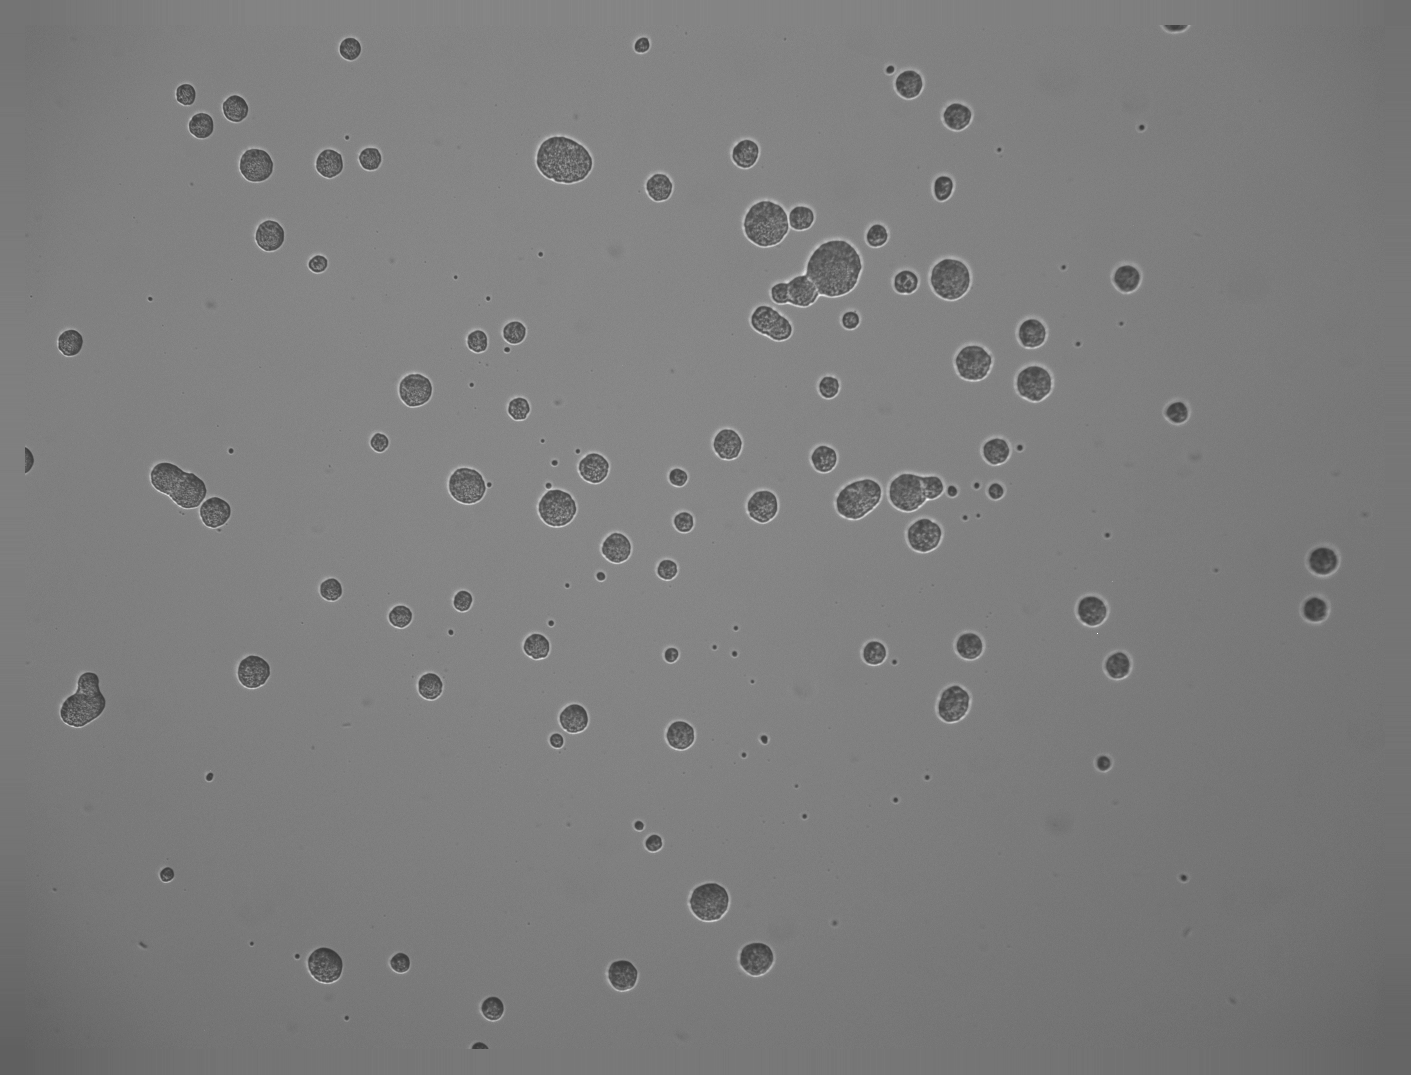
\includegraphics[height=\paperheight,width=\paperwidth]{FinishingCells.png}};
}
\begin{frame}
\titlepage % Print the title page as the first slide
\end{frame}
\usebackgroundtemplate{ }

%----------------------------------------------------------------------------------------
%	PRESENTATION SLIDES
%----------------------------------------------------------------------------------------

\begin{frame}
\frametitle{Microbial Growth Models}
\begin{figure}
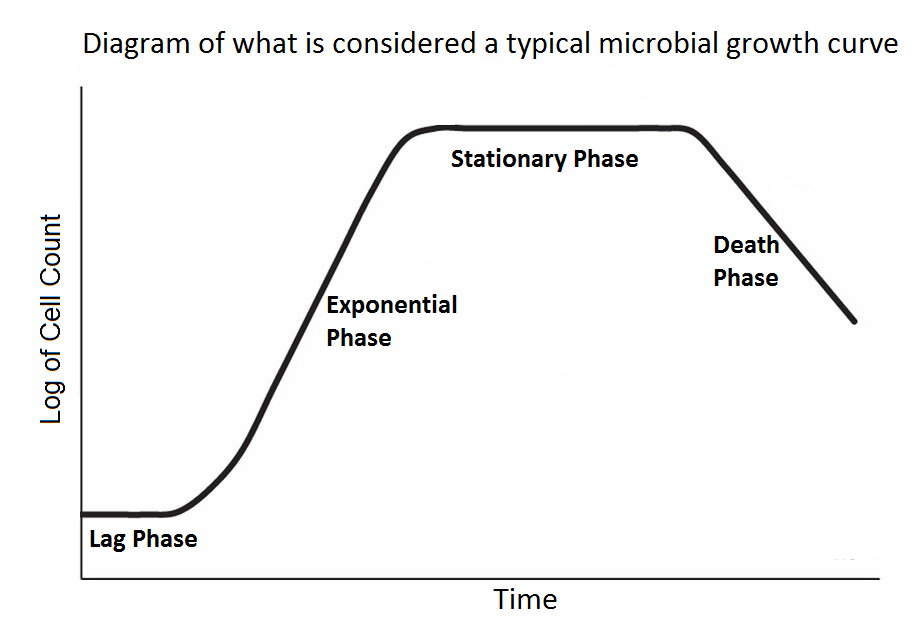
\includegraphics[width=0.8\linewidth]{GrowthPhases.png}
\end{figure}
\end{frame}
%we will focus on the first two stages; least explored
%apoptosis has received much attention in micro-biology
%lag phase is like the hufflepuff of harry potter; no one seems to care about it but there might actually be some really cool magic going on... at least that's what I'm going to try and convince you of in the next few minutes 

\begin{frame}
\frametitle{Setting the Scene}
\begin{block}{Growth Rate}
A measure of how quickly cells are progressing through the cell cycle
\end{block}
\vspace{+1em}
\begin{itemize}
\item Key model parameter when capturing population dynamics
\item Important component of evolutionary fitness
\item Subject to great selective forces
\item Applications in food security, microbial infection modeling, tumorigenesis dynamics, etc.
\end{itemize}
\end{frame}
%Here, talk a bit about experimental design and how this has become high-throughput 
%uQFA data 

\begin{frame}
\frametitle{Research Problem}
\vspace{-2em}
\begin{figure}
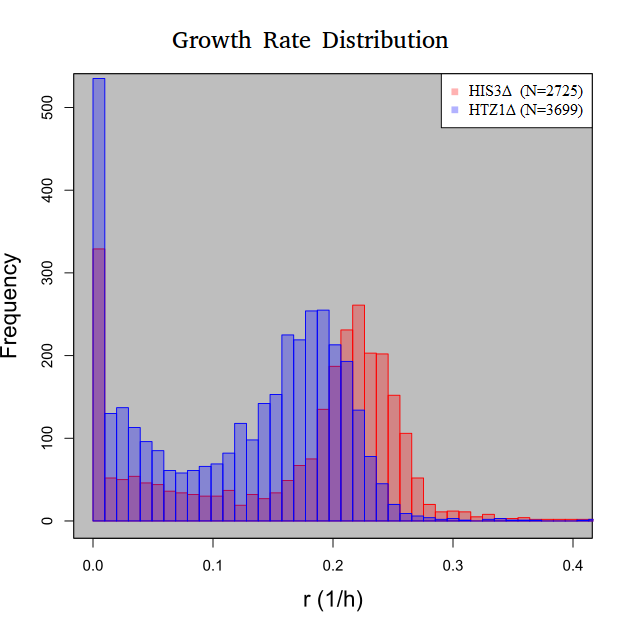
\includegraphics[width=0.4\linewidth]{GrowthRateDistr.png}
\end{figure}
\vspace{-2em}
\begin{block}{Growth rate is typically measured at the population scale.}
\begin{itemize}
\item Assume that observations at that scale apply to \textbf{individual cells}.
\item Assume that all members of the population behave in the same way... 
\item Increasing evidence that, even among isogenic populations, there is considerable heterogeneity in growth rates.
\end{itemize}
\end{block}
\end{frame}

% \begin{frame}
% \frametitle{Research Problem}
% \begin{center}
% \begin{tikzpicture}
%   \node (slide1) {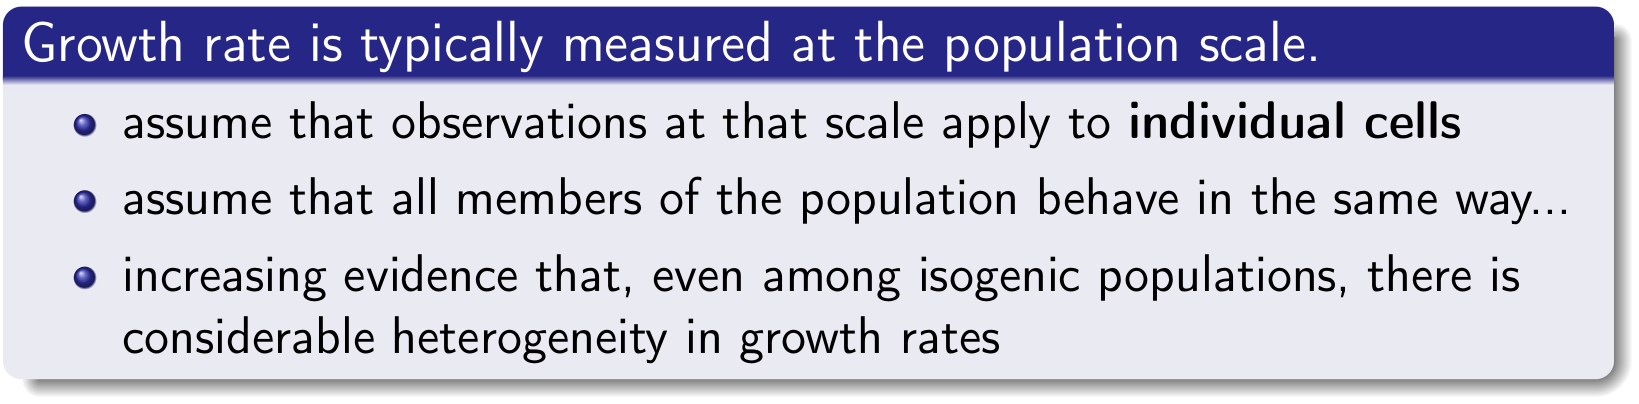
\includegraphics[width=1\linewidth]{GrowthRateText.png}};
%   \pause
%   \node (slide2) {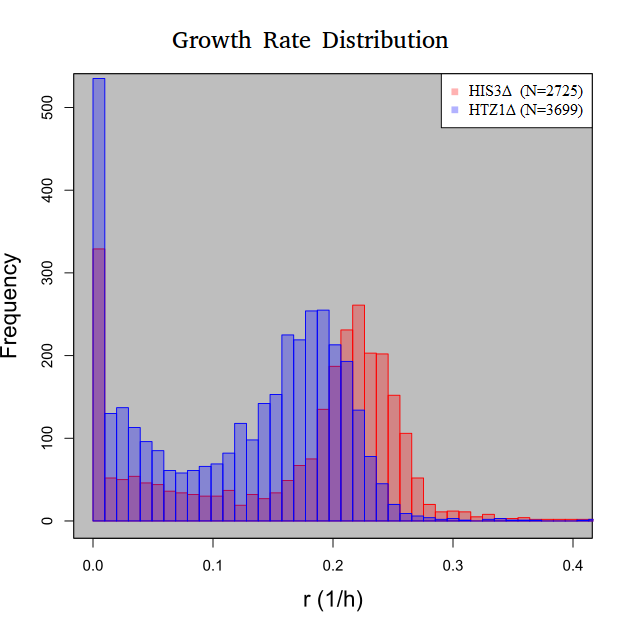
\includegraphics[width=0.6\linewidth]{GrowthRateDistr.png}};
% \end{tikzpicture}
% \end{center}
% \end{frame}

%Now this idea of heterogeneity in growth rate among genetically identical cells actually ties in very nicely with some of the observations Dr Lawless made in the lab 
\begin{frame}
\frametitle{Prior Observations}
\begin{block}{$\mu$QFA data by Lawless:}
\begin{itemize}
\item Little evidence for a lag phase when looking at individual lineages. 
\item Cells divide almost immediately, with some clones dividing more quickly than others. 
\end{itemize}
\end{block}
\vspace{-0.5em}
\begin{figure}

\includegraphics[width=0.07\linewidth]{BlueArrow.png}
\end{figure}
\vspace{-0.5em}
\begin{block}{}
\begin{itemize}
\item It may thus be plausible that population-level observations of a lag phase are the results of competition between clonal cell lineages. 
\item We hope to demonstrate that the lag phase can be \textbf{apparent at the population level}, despite being \textbf{absent at the single cell level}, due to inter-lineage variability in growth rate.
\end{itemize}
\end{block}
\end{frame}
%so in order to address this issue we decided to get hold of some data
%.... a lot of data 
%red is the healthy and blue the sicker strain 

\begin{frame}
\frametitle{Data, data and more data}
Data sets which will be used to capture growth rate heterogeneity: 
\begin{enumerate}
\item $\mu$QFA data produced by Lawless (unpublished),
\item High-throughput microscopy assay data by Levy et al. 2012,
\item High-throughput microscopy assay data by Ziv et al. 2013.
\end{enumerate}
\vspace{+1em}
\begin{figure}
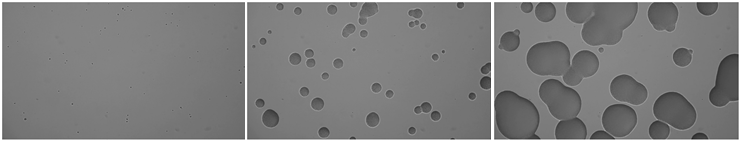
\includegraphics[width=1\linewidth]{CellGrowth3Pic.png}
\end{figure}
\end{frame}

\begin{frame}
\frametitle{Proposed Research: Aims}
\begin{itemize}
\item Find a model which best captures heterogeneity in microbial growth curves through \textbf{single lineage observations}.
\item Explore the implications which such a model may have on the interpretation of various growth phases.
\item Repeat the $\mu$QFA experiments with the aim of validating model predictions.
\end{itemize}
\begin{center}
\begin{tikzpicture}
	\node (slide1) {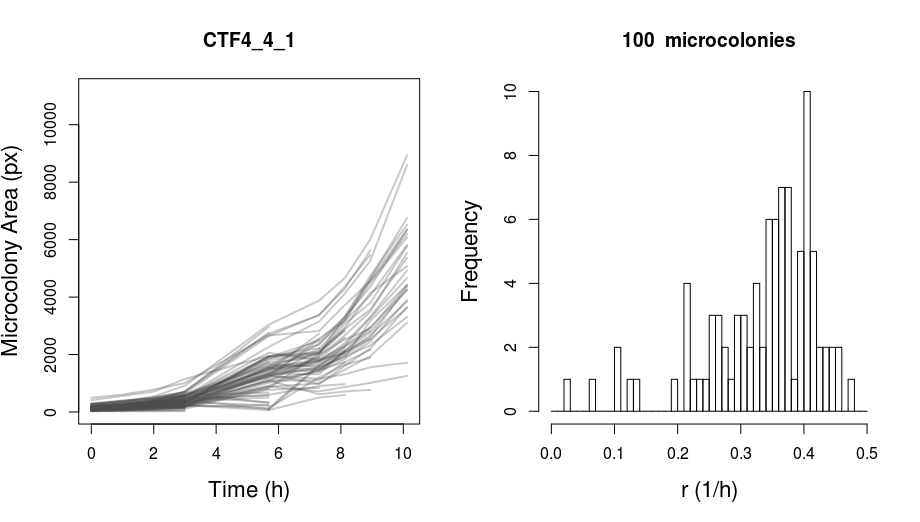
\includegraphics[width=0.65\linewidth]{LevyExampleOutput.png}};
    \pause
    \node (slide2) {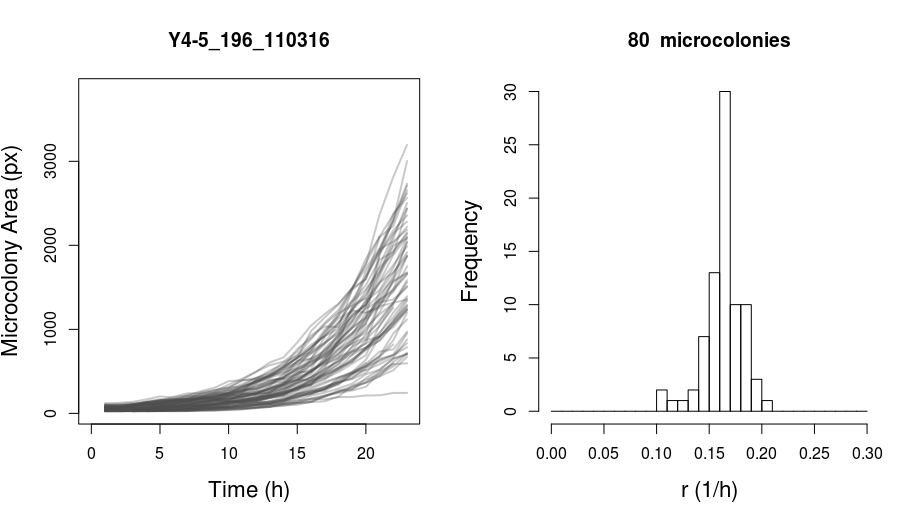
\includegraphics[width=0.65\linewidth]{ZivExampleOutput2.png}};
    \pause
    \node (slide3) {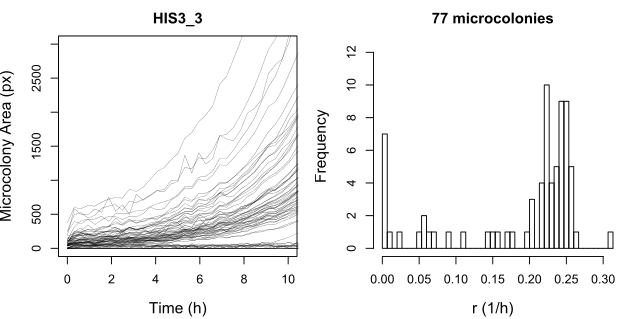
\includegraphics[width=0.68\linewidth]{LawlessExampleOutput.png}};
\end{tikzpicture}
\end{center}
\end{frame}
%Novelty will arise from the fact that individual cells lineages will be analyzed separately, which will allow for us to explore inherent heterogeneities. 
%As outlined, novelty lies in that we will consider single cell lineages to explore population intrinsic heterogeneities.

\begin{frame}{Proposed Research:Objectives}
    \begin{columns}[c] % the "c" option specifies center vertical alignment
    \column{.5\textwidth} % column designated by a command
    \begin{itemize}
		\item Data accessibility 
% 		\begin{itemize}
% 		\item Parser \& calibration curves
% 		\end{itemize}
    \item Model development
% 		\begin{itemize}
% 		\item Deterministic, stochastic, hybrid
% 		\end{itemize}
	\item Parameter inference workflows
% 		\begin{itemize}
% 		\item Likelihood-free parameter inference techniques
% 		\item \texttt{pyMC, smfsb, ...}
% 		%pyMC for deterministic modelling; smfsb for particle MCMC as described by Wilkinson 
% 		%PyMC is a python module that implements Bayesian statistical models and fitting algorithms, including Markov chain Monte Carlo.
% 		\end{itemize}
    \end{itemize}
    
    \column{.5\textwidth}
    \begin{itemize}
    \item Model fit 
% 		\begin{itemize}
% 		\item BIC or Bayes Factors
% 		\end{itemize}
		%eat your own dog food
	\item Mechanistic insights
% 		\begin{itemize}
% 		\item Analyze the lag phase
% 		\item Analyze the effect of sampling
% 		\item Further experiments?
% 		\end{itemize}
	\item Submission
% 		\begin{itemize}
% 		\item \textit{arXiv} and possible journal submission
% 		\end{itemize}
	\end{itemize}
    \end{columns}
\vspace{+3em}
\begin{block}{
%Types of Models?
\begin{itemize}
\item Logistic deterministic model; 
\item Standard Gillespie stochastic model; 
\item Hybrid model combining deterministic and stochastic models.
\end{itemize}}
%Biologically Meaningful Models?
\begin{itemize}
\item birth-only models
\item lower bound for time sampling
\item switch to a non-dividing stage 
\end{itemize}
\end{block}
\end{frame}

% We will explore likelihood-free parameter inference techniques in order to obtain growth rate and carrying capacity parameters from each of the data sets. Various options such as \verb pyMC for deterministic modeling, or the particle MCMC described by \citealp{Wilkinson06}, for stochastic modeling, are available foundations to work off. 
\usebackgroundtemplate{%             declare it
\tikz[overlay,remember picture] \node[opacity=0.3, at=(current page.center)] {
   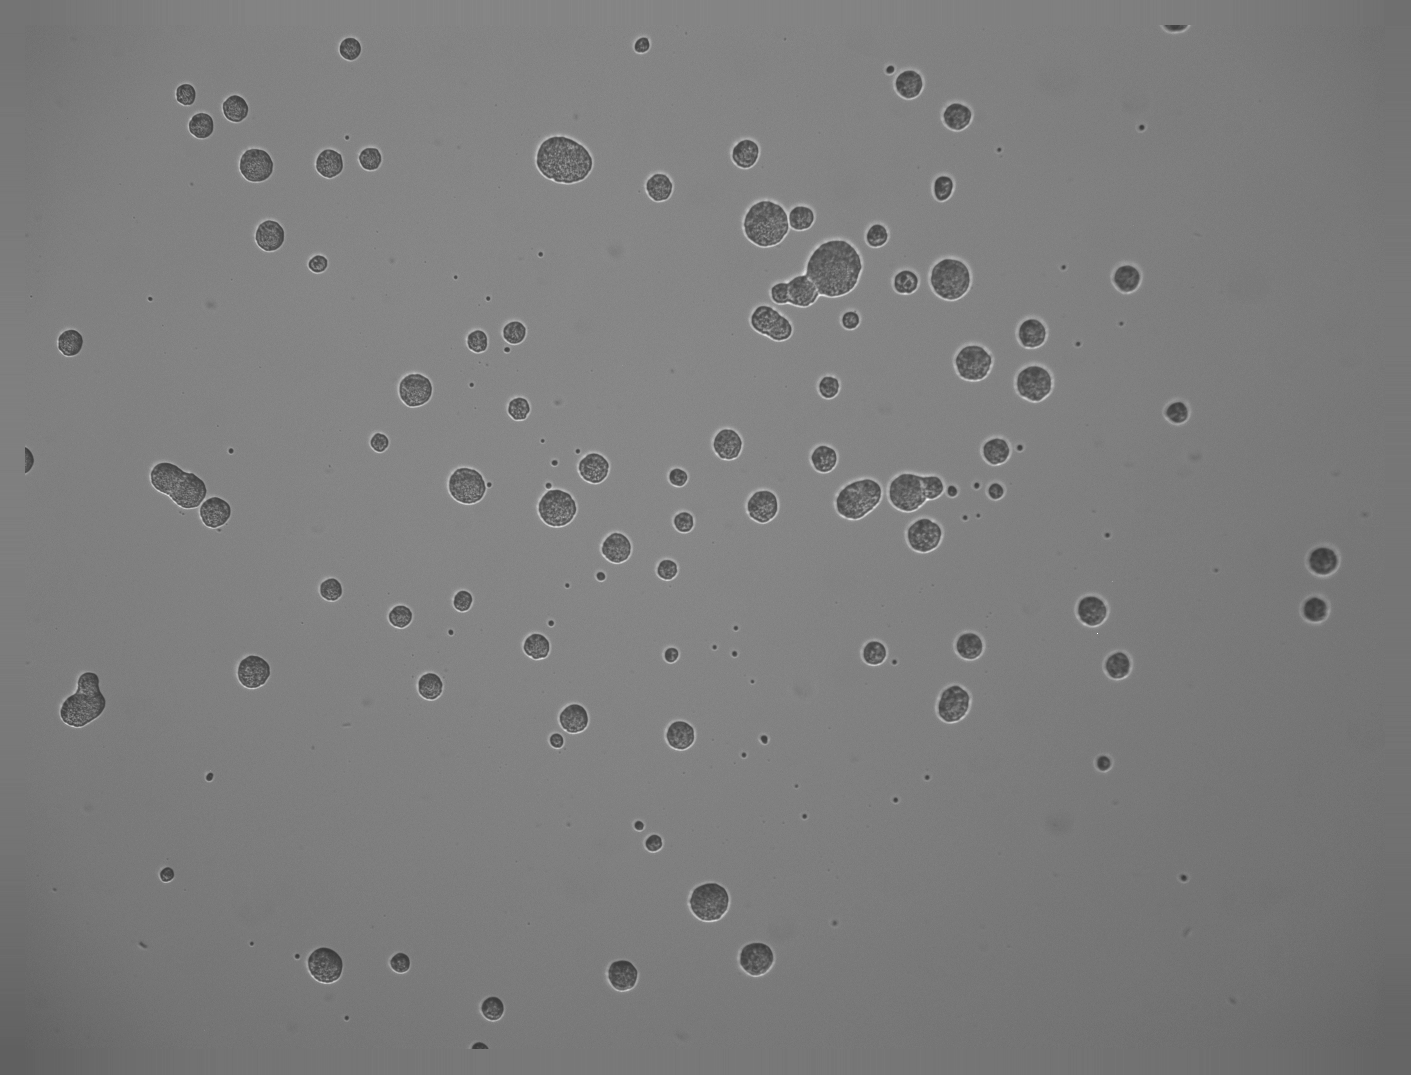
\includegraphics[height=\paperheight,width=\paperwidth]{FinishingCells.png}};
}
\begin{frame}
\frametitle{Summary}


Can we find a stochastic model that \textbf{reduces the apparent heterogeneity} of growth rates in data? \\~\\
\vspace{+1em}
Does explicit modeling of cell lineages give rise to an \textbf{apparent lag phase} at the population level? \\~\\
\vspace{+1em}
How is \textbf{sampling} from different phases affected by heterogeneity? 
\end{frame}
\usebackgroundtemplate{ }

\begin{frame}
\frametitle{Research Significance}
\begin{block}{Microbiology is progressing to become a data-rich science}
\begin{itemize}
\item Limiting factors in scientific advances often no longer rest in the amount of available data...
\item ...but in the quantitative analyses performed on them.
\item This project makes efficient use of a vast range of \textbf{existing, expensive, experimental} data sets.
\end{itemize}
\end{block}
\begin{block}{Single-lineage stochastic, deterministic and hybrid models}
\begin{itemize}
\item First time that these models will be considered along-side each other.
\item If we are be able to reduce the apparent heterogeneity in population parameters...
%by considering single lineage variations in clonal cell cultures...
\item ...the explored mechanistic implications and the developed models will have \textbf{vast applications} (e.g. experimental design, risk assessments, tumorigenesis, etc.).
\end{itemize}
\end{block}
\end{frame}

\begin{frame}
\frametitle{Any Questions?}
\vspace{-0.8em}
\begin{figure}
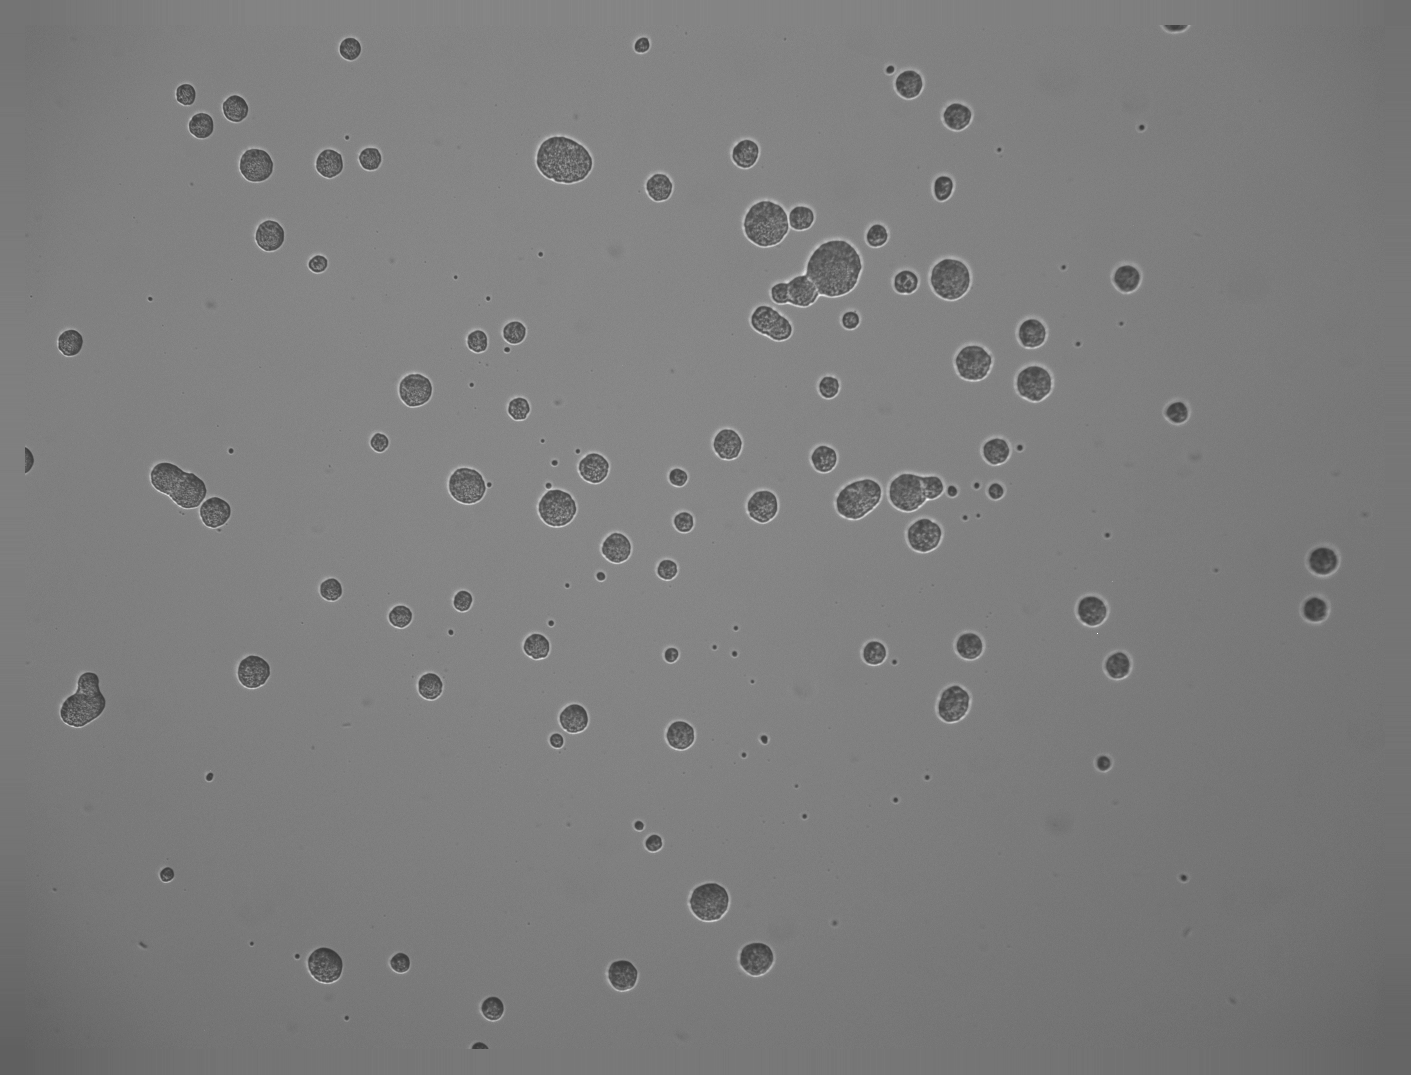
\includegraphics[width=0.9\linewidth]{FinishingCells.png}
\end{figure}
\end{frame}


\end{document}